%%%%%%%%%%%%%%%%%%%%%%%%%%%%%%%%%%%%%%%%%%%%%%%%%%%%%%%%%%%
% --------------------------------------------------------
%  _____           
% |_   _|_ _ _   _ 
%   | |/ _` | | | |
%   | | (_| | |_| |
%   |_|\__,_|\__,_|
%
% LaTeX2e Template
% Version 2.6.0 (21/04/2026)
%
% Author: 
% Guillermo Jimenez (memo.notess1@gmail.com)
% 
% License:
% Creative Commons CC BY 4.0
% --------------------------------------------------------
%%%%%%%%%%%%%%%%%%%%%%%%%%%%%%%%%%%%%%%%%%%%%%%%%%%%%%%%%%%
% --------------------------------------------------------
% Github Repository:
% https://github.com/MemoJimenez/Tau-class
% --------------------------------------------------------
%%%%%%%%%%%%%%%%%%%%%%%%%%%%%%%%%%%%%%%%%%%%%%%%%%%%%%%%%%%

\documentclass[9pt,a4paper,twocolumn,twoside]{tau-class/tau}
\usepackage[english]{babel}

% Spanish babel recomendation
% \usepackage[spanish,es-nodecimaldot,es-noindentfirst]{babel} 

%----------------------------------------------------------
% Title & Authors/Affiliations
%----------------------------------------------------------

\doctype{CS240 Proposal}
\title{Budgeted Value-Connection Model for Shanghai Metro Line Planning}

%----------------------------------------------------------

\author[a,1]{Yuzhou Lu}
\author[a,2]{Zaizhou Yang}
\author[a,3]{Jingrong Guan}

%----------------------------------------------------------

\affil[a]{ShanghaiTech University}

%----------------------------------------------------------
% Document-, Footer- information
%----------------------------------------------------------

\dates{This manuscript was compiled on \today}

\docinfo{CS240 project proposal on graph optimization for urban rail transit planning.} 

%----------------------------------------------------------

\footinfo{CS240 Proposal}
\theday{\today}
\organization{ShanghaiTech University}
\leadauthor{Y. Lu et al.}

%----------------------------------------------------------
% Abstract and Keywords
%----------------------------------------------------------

\begin{abstract}    
    This project studies a graph-optimization formulation for Shanghai metro line planning. We first generate a set of candidate stations from residential population, estimated jobs, fixed transport hubs, and large commercial centers. Each candidate station has a spatial coordinate and a scalar value. Given a total construction-length budget, the planning task is to connect a subset of these stations so that the total reward of connected station pairs is maximized. The reward between two connected stations is modeled as the product of their values divided by their shortest-path distance in the selected metro network, which favors connecting high-value station pairs through spatially efficient routes. The goal is to generate candidate rail corridors that are interpretable, computationally tractable, and compatible with practical planning constraints.
\end{abstract}

%----------------------------------------------------------

\keywords{transit network design problem, budgeted network design, metro planning, candidate stations, Shanghai}

%----------------------------------------------------------

\begin{document}
		
    \maketitle 
    \thispagestyle{firststyle}
    
%----------------------------------------------------------

\section{Topic Selection}

    \taustart{N}etwork design is one of the most strategic stages in urban rail transit planning. The spatial structure of a metro network determines which areas can be reached directly, where transfers are required, and how efficiently passenger demand can be served. It also constrains later operational decisions such as frequency setting, timetable design, vehicle scheduling, and crew scheduling. Therefore, before optimizing detailed operations, planners must first decide where lines should be placed and which urban areas they should connect \cite{owais2026tndp}.

    This planning challenge is commonly studied as the Transit Network Design Problem (TNDP). In general, TNDP aims to determine a set of transit routes, and sometimes their service frequencies, that balances the interests of operators and passengers. Operators prefer lower construction and operating costs, while passengers prefer shorter travel time, fewer transfers, and more equitable service coverage. These objectives often conflict with one another, making TNDP a multi-objective, constrained, and computationally difficult problem \cite{owais2026tndp}.

    In this project, we focus on a selected study area in Shanghai and investigate a simplified but meaningful version of metro line planning. We first construct candidate stations from residential population, estimated jobs, fixed transport centers, and large commercial centers. Each candidate station has a coordinate and a scalar value. Under a total line-length budget, the task is to choose a connected line or network that links high-value stations efficiently. This gives a budgeted graph-optimization problem related to orienteering, prize-collecting network design, and Steiner-tree-style connection heuristics, while keeping the model directly tied to observable urban data.

    Our goal is not to replace full-scale professional transit planning, but to build an explainable algorithmic framework for candidate line generation. The current model uses station value as a proxy for potential demand and rewards connected station pairs by value product divided by their shortest-path distance inside the selected network. This lets us connect a classical graph problem with a realistic urban-planning scenario while keeping the project scope suitable for implementation and evaluation.

\section{Related Work}

    Laporte et al. study the location of a single rapid-transit alignment as a maximal trip-coverage problem \cite{laporte2005tripcoverage}. Their input consists of candidate station nodes, an origin-destination demand matrix, population-density and catchment information around stations, walking-distance measures, competing automobile travel times, and a maximum alignment length. The output is one rapid-transit alignment, represented as an ordered set of selected stations. The main assumptions are that demand can be captured when both ends of an OD pair are served by the alignment, and that the attractiveness of transit relative to car travel can be estimated through a logit mode-choice function. The key constraints are a maximum line length, station selection from a discrete candidate set, and a non-self-intersecting alignment. Because the resulting problem is NP-hard, the paper uses constructive heuristics, including greedy extension, greedy insertion, and post-optimization. This work is the closest single-line reference for our project: our model also searches over candidate stations under a length budget, but replaces explicit OD demand by a value-product proxy when a surveyed OD matrix is unavailable.

    Chai et al. formulate urban rail network design under road-network, trip-demand, and land-use constraints \cite{chai2019urbanrail}. Their input includes a basic network derived from urban roads and main passenger-flow corridors, candidate stations and sections, OD passenger demand, trip production and attraction by traffic zone, land-use intensity, station coordinates, section lengths, section capacities, and planning bounds on line length, number of stations, and number of lines. The output is a set of rail lines forming an urban rail transit network. The model assumes that a reasonable rail network should match both the spatial distribution of travel demand and the spatial distribution of land-use intensity, while also avoiding inefficient transfers. Its constraints include line topology, station and section repetition limits, OD flow conservation, demand and land-use matching thresholds, section capacities, network-size bounds, and minimum turning angles between adjacent sections. The method first builds a restricted basic network, defines station-importance and matching indices, and then solves the NP-hard model using a simulated-annealing neighborhood search. Compared with this full network-design formulation, our project keeps the same spirit of spatially constrained rail planning but simplifies the inputs to candidate-station values and construction length, making the algorithm easier to implement and evaluate within the course scope.

    Ahmed et al. propose an integrated GIS and genetic-algorithm framework for rail transit system planning \cite{ahmed2020gisga}. Their input contains GIS layers such as land use, existing transport networks, census population, land values, topography, environmental exclusion zones, OD trip matrices, candidate station feasibility grids, planner-specified terminal station pairs, desired topology, and construction and operation cost parameters. The output is a joint station-location and line-network plan. The model assumes that station feasibility can be screened before optimization from spatial, demographic, economic, environmental, and topological criteria, and that station selection and line layout should be optimized together rather than sequentially. The constraints include lower and upper bounds on the number of stations per line, station spacing, required transfer or intersecting stations, maximum overlap between lines, environmental exclusions, and feasibility thresholds for candidate station cells. The method uses GIS preprocessing to define the feasible search space and a genetic algorithm to optimize the combined plan, with Dijkstra shortest paths used inside the fitness evaluation. This paper motivates our preprocessing pipeline: we similarly construct candidate stations from population, jobs, transport hubs, and commercial centers before running graph optimization, but use a smaller budgeted value-connection objective instead of a full life-cycle cost model.

\section{Data Collection}

    The data pipeline is implemented in \inlinecode{transit\_pipeline/line\_network\_model}. It first prepares demand-related spatial layers, and then converts them into four types of candidate station centers: residential population centers, estimated job centers, fixed transport centers, and large commercial centers. The current study area is a central Shanghai bounding box
    \[
        (121.40, 31.14, 121.56, 31.26),
    \]
    in the order west, south, east, north. The total population inside this area is normalized to $3{,}000{,}000$ people. All intermediate and final products are written under \inlinecode{line\_network\_model/output}, so every station used by the optimization model can be traced back to the preprocessing files.

    The first stage, \inlinecode{00\_prepare\_demand\_data.py}, downloads and caches OpenStreetMap data through Overpass. The query collects building footprints, roads, house-number nodes, selected land-use polygons, amenities, leisure features, shops, tourism features, railway and public-transport tags, and airport-related features. In the current run, this produced 476,358 raw OSM elements. From these elements, the script extracted 41,859 building polygons, 17,873 residential buildings with estimated flats, 60,321 functional-category points or areas, 11,324 work destinations, and 2,065 activity attractions. The prepared files include \inlinecode{04\_population\_points.geojson}, \inlinecode{05\_function\_categories.geojson}, \inlinecode{06\_work\_destinations.geojson}, and \inlinecode{07\_activity\_attractions.geojson}.

    The residential population layer is derived from OSM building footprints. Buildings are removed if their centroid falls inside excluded land-use or amenity areas, where excluded land uses are allotments, commercial, industrial, military, and retail, and excluded tag families include amenity and leisure. For the remaining residential buildings, the number of flats is estimated from \inlinecode{building:flats} when available. Otherwise, single homes such as \inlinecode{house} and \inlinecode{detached} receive one flat, apartment-like buildings such as \inlinecode{apartments}, \inlinecode{residential}, \inlinecode{terrace}, and \inlinecode{semidetached\_house} use house-number counts when available, and building levels multiply the estimated flats. A fixed random seed of 42 distributes the normalized population of $3{,}000{,}000$ across all estimated flats, giving one population-weighted point per residential building centroid. These points are then clustered into 29 residential population centers using weighted $k$-means, with population as the sample weight.

    The job layer is estimated from functional OSM categories rather than from surveyed employment data. Functional features are classified with a priority order: healthcare, education, transport or public facilities, hotel and tourism, retail and service, commercial and office, industry, leisure and park, residential, and other. Work destinations are created only for categories that plausibly generate employment: commercial and office, retail and service, industry, education, healthcare, and hotel and tourism. The job estimate uses category-specific default building levels, square meters per job, and minimum base jobs. For example, commercial and office features use 6 default levels, 25 square meters per job, and at least 8 jobs; retail and service uses 2 levels, 35 square meters per job, and at least 6 jobs; healthcare uses 6 levels, 45 square meters per job, and at least 35 jobs. These 11,324 job destinations are clustered into 18 job centers using weighted $k$-means, with estimated jobs as the weight.

    The transport-center layer is extracted from the functional-category file using railway, public-transport, and airport-related tags. To avoid treating every subway entrance as a strategic hub, the current configuration only keeps named major centers through a manual alias table: Shanghai Railway Station, Shanghai South Railway Station, and Longyang Road. These centers receive fixed values of 300,000, 260,000, and 220,000 respectively. They are influential candidate centers but are not mandatory stops, because \inlinecode{TRANSPORT\_CENTERS\_REQUIRED} is set to false. In the current run, three rail-hub candidates were found and no airport hub was included inside the study area.

    The commercial-center layer comes from activity attractions. Retail and service features are treated as large commercial centers only when their name ends with the configured suffixes for plaza or shopping center. Each retained commercial hub receives a fixed value of 30,000. The same activity-attraction file also records tourism and leisure attractions, with weights based on area, but these tourism points are used only as context in the current visualization and are not converted into fixed station centers. The current run found 57 raw commercial hub candidates and 2,008 tourism attractions.

    The second stage, \inlinecode{01\_select\_stations.py}, merges the four center layers into the final candidate station set. All population, job, transport, and commercial centers are pooled together. Centers within 1,000 meters are merged into a single candidate station, located at the value-weighted centroid of its components. The station value is additive:
    \[
        v_i =
        v_i^{\mathrm{pop}} +
        v_i^{\mathrm{job}} +
        v_i^{\mathrm{trans}} +
        v_i^{\mathrm{comm}}.
    \]
    This merge radius also acts as the minimum station-spacing rule. In the current output, 29 population centers, 18 job centers, 3 transport centers, and 57 commercial centers are merged into 54 candidate stations, with a minimum pairwise spacing of 1,010.4 meters. The summed station value is 9,776,462.8, consisting of 3,000,000 population value, 4,286,462.8 job value, 880,000 transport value, and 1,710,000 commercial value. The final station table \inlinecode{01\_candidate\_stations\_table.csv} stores each station's coordinates, source layers, component count, component values, total value, and name.

    A separate reference step, \inlinecode{02\_fetch\_existing\_metro\_reference.py}, downloads existing subway, light-rail, and monorail geometries and subway stations from Overpass inside the same bounding box. These existing metro lines are not used as mandatory inputs to the current optimization objective, but they provide a spatial reference layer for checking whether the generated candidate network is plausible relative to the real Shanghai rail system.

\section{Problem Formulation}

    We formulate the planning task as a budgeted value-connection problem on a spatial graph. The input of the optimization stage is a set of candidate stations
    \[
        V = \{1,2,\ldots,n\}.
    \]
    Each candidate station $i \in V$ has a coordinate $p_i=(\lambda_i,\phi_i)$ and a nonnegative value $v_i$. In our implementation, these candidate stations are obtained from four preprocessing layers: residential population centers, estimated job centers, fixed transport hubs, and large commercial centers. When multiple layer centers are within one kilometer, they are merged into one candidate station by a value-weighted centroid, and their component values are added. Thus,
    \begin{equation}
        v_i =
        v_i^{\mathrm{pop}} +
        v_i^{\mathrm{job}} +
        v_i^{\mathrm{trans}} +
        v_i^{\mathrm{comm}} .
    \end{equation}
    The file \inlinecode{01\_candidate\_stations\_table.csv} records these components for every candidate station.

    We construct a complete candidate graph $G=(V,E)$, where each candidate edge $e=(i,j) \in E$ has construction length $\ell_{ij}$, measured by the geographic distance between its two endpoint stations. The planning decision is not only to select a set of edges, but to select a set of metro lines
    \begin{equation}
        \mathcal{L}=\{L_1,L_2,\ldots,L_K\}.
    \end{equation}
    Each line $L_k$ is an ordered sequence of candidate stations. It may be an open line, such as $(s_1,s_2,\ldots,s_m)$, or a closed loop line, such as $(s_1,s_2,\ldots,s_m,s_1)$. Therefore, cycles are allowed in the planned network. The selected metro subgraph $S=(V_S,E_S)$ is the union of all stations and edges used by the lines in $\mathcal{L}$. Let $x_{ij} \in \{0,1\}$ indicate whether edge $(i,j)$ is selected by at least one line, $y_i \in \{0,1\}$ indicate whether station $i$ is included, and $z_{ij} \in \{0,1\}$ indicate whether stations $i$ and $j$ are both included in the same connected selected network.

    For any two selected stations $i,j \in V_S$, let $D^S_{ij}$ denote the shortest-path distance between $i$ and $j$ within the selected metro subgraph $S$, where the length of a path is the sum of the construction lengths $\ell_e$ of all selected edges $e$ on that path. Thus $D^S_{ij}$ is not the direct geographic distance between $i$ and $j$ unless the selected network contains a direct edge between them. The key modeling assumption is that connecting two high-value stations is more beneficial when they are close in the planned metro network. Therefore, if stations $i$ and $j$ are included in the same connected planned line or network, their pairwise reward is defined as
    \begin{equation}
        r_{ij}(S) = \frac{v_i v_j}{D^S_{ij}}, \qquad i,j \in V_S,\ i<j .
    \end{equation}
    This term acts as a simplified OD-demand proxy. The product $v_i v_j$ captures the idea that trips are more likely between two strong demand centers, while the division by $D^S_{ij}$ favors planned networks in which valuable station pairs can reach each other through short metro paths.

    To discourage unrealistic rail alignments, we introduce a line-level turn-angle penalty. This penalty is computed along each ordered line rather than from the unordered adjacency structure of the selected subgraph. For every consecutive triple of stations $(a,b,c)$ on the same line, let $\theta_{abc}$ denote the deflection angle at station $b$, where $\theta_{abc}=0^\circ$ corresponds to a straight continuation and larger values correspond to sharper turns. For a closed loop line, triples are evaluated cyclically across the connection from the last station back to the first station. For an open line, only interior stations contribute to the turn penalty; terminal stations do not.
    \begin{equation}
        P(\mathcal{L}) =
        \sum_{L_k \in \mathcal{L}}
        \sum_{(a,b,c)\in T(L_k)}
        \left(
        \frac{\max(0,\theta_{abc}-\theta_0)}{90}
        \right)^2 .
    \end{equation}
    In the implementation we use $\theta_0=60^\circ$ and a penalty coefficient $\lambda=120{,}000{,}000$. Under a total length budget $B$, the objective is
    \begin{equation}
        \max \quad
        \sum_{\{i,j\}\subseteq V}
        \frac{v_i v_j}{D^S_{ij}} z_{ij}
        - \lambda P(\mathcal{L})
    \end{equation}
    subject to
    \begin{equation}
        \sum_{(i,j)\in E} \ell_{ij} x_{ij} \leq B,
    \end{equation}
    \begin{equation}
        z_{ij} \leq y_i,\qquad
        z_{ij} \leq y_j,\qquad
        \forall i,j \in V,\ i<j,
    \end{equation}
    together with consistency constraints requiring that every selected edge belongs to at least one line in $\mathcal{L}$ and that every selected station with $y_i=1$ appears on at least one selected line. The union subgraph $S$ may contain cycles, either because an individual line is a closed loop or because multiple lines jointly create a cycle. If the model is restricted to a single open line, then the result is a path; if closed or multiple lines are allowed, the result can be a cyclic rail network.

    Some candidate stations, such as Shanghai Railway Station, Shanghai South Railway Station, and Longyang Road, are fixed transport centers. In the current implementation they are represented as high-value candidate stations, but they are not mandatory stops. Large commercial centers are treated similarly: they are fixed candidate stations with fixed commercial value, but the algorithm is not forced to visit every one of them. This keeps transport hubs and commercial centers influential in the objective while allowing the length budget and turn-angle penalty to decide whether they should actually be selected.

    In words, the model asks: given candidate stations with coordinates and values, and a maximum construction length, which set of open or closed metro lines should be built so that the connected high-value station pairs produce the largest total reward while avoiding excessive local turns along each line? This formulation keeps the project close to classical network design, orienteering, and budgeted prize-collecting problems, while avoiding the need for a surveyed OD matrix at this stage.


\iffalse
    This class includes the following files in the tau-class folder:
	
	\begin{itemize}
		\item \inlinecode{tau.cls} — The main class file.
		\item \inlinecode{tauenvs.sty} — A package containing custom environments.
		\item \inlinecode{taubabel.sty} — A support package for multilingual.
		\item \inlinecode{README.md} — With essential information.
	\end{itemize}

    Additionally, this template includes a sample document \inlinecode{main.tex}, a bibliography file \inlinecode{tau.bib}, as well as figures, tables and code examples to help you get started quickly.

    \subsection{License}
    
        This work is the creation of Guillermo Jimenez licensed under Creative Commons CC BY 4.0. You may adapted, shared and distributed your work, ensuring that proper credit is given to the original author.

\fi
\section{Document Styling}

    \subsection{Document Type}

        Before the main title, a brief descriptor indicates the type of document (e.g., Lab Report, Research Article, etc). This is controlled by the \inlinecode{\doctype{}} command. 
        
        If no such label is needed, omit the command and the title will automatically reposition itself to maintain proper vertical spacing and visual alignment.

    \subsection{Abstract and Keywords}

        The abstract and keywords are declared in the preamble of the document, before the beginning of the document, and are automatically positioned during the title creation process.

    \subsection{Lettrine}

		The \inlinecode{\taustart{}} command, provides a personalized lettrine for the beginning of the first paragraph as shown in this example.

	\subsection{Table of Contents}

        This class includes a customized design for the table of contents, which is disabled by default. To enable it, insert the \inlinecode{\tableofcontents} command before your first section.

    \section{Cross-Reference Commands*}

        Tau-class provides shorthand commands for cross-referencing figures, tables, code listings, and equations. To customize the label format, edit the \inlinecode{taubabel.sty} file. Label translations for Spanish are handled automatically.

        \begin{itemize}
            \item \inlinecode{\figref{}} — Uses the label style defined by \inlinecode{\figlabel}.
            \item \inlinecode{\figsref{}} — Uses the label style defined by \inlinecode{\figslabel}.
            \item \inlinecode{\tabref{}} — Uses the label style defined by \inlinecode{\tablabel}.
            \item \inlinecode{\coderef{}}  — Uses the label style defined by \inlinecode{\captionlabelcode}.
            \item \inlinecode{\equref{}} — Uses the label style defined by \inlinecode{\eqlabel}.
        \end{itemize}
        
         These commands generate fully hyperlinked references, both the label and the number, ensuring navigation to the referenced element when clicked in the PDF.

\section{Figures and Tables}

    \subsection{Figures}
		
    	\figref{fig:figure} shows a 3D surface plot of the hyperbolic paraboloid $z=x^2-y^2$.
    		
    	\begin{figure}[H]
    		\centering
    		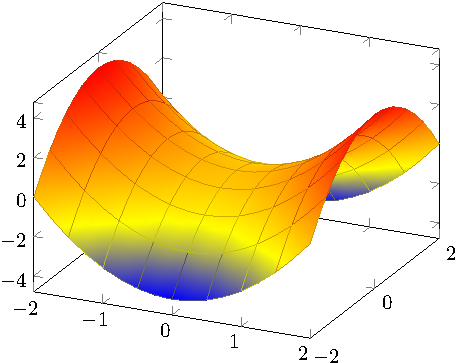
\includegraphics[width=0.75\columnwidth]{figures/Example.pdf}
    		\caption{Hyperbolic paraboloid obtained from PGFPlots \cite{PFGPlots}.}
    		\label{fig:figure}
    	\end{figure}

    \subsection{Tables}
	
        \tabref{tab:table} shows an example table of some astronomical objects. 

        \begin{table}[H]
        	\caption{Astronomical Object Data}
        	\label{tab:table}
        	\begin{tabular}{
        		>{\raggedright\arraybackslash}p{0.25\columnwidth}
        		>{\raggedright\arraybackslash}p{0.30\columnwidth}
        		>{\raggedright\arraybackslash}p{0.31\columnwidth}
        	}
        	\toprule
        	\textbf{Object} & \textbf{Type} & \textbf{Distance (Light Years)} \\
        	\midrule
        	Alpha Centauri & Star system & 4.37 \\
        	Betelgeuse & Red supergiant star & 642.5 \\
        	Andromeda & Spiral galaxy & 2.537 million \\
        	Earth & Planet & 0 \\
        	Sirius & Binary star system & 8.6 \\
        	\bottomrule
        	\end{tabular}
        	\tabletext{Note: The table contains data of some famous celestial objects.}
        \end{table}

        The \inlinecode{\tabletext{}} command is used to add notes to tables easily. 

\section{Document Data}

    \subsection{Front-Matter Footer Block*}

        The \inlinecode{\docinfo{}} command inserts a dedicated block at the bottom of the first column. Unlike floating elements, this block stays fixed in place — positioned visually like a footnote, although technically it is not one.
    
        The \inlinecode{\docinfo{}} block was created to give you greater control over supplementary document data, such as publication dates, licensing information, extended author details, and other front-matter notes. You can fully customize its content to suit your needs. If it’s not required, omit the command to remove this block entirely.
    
        \begin{note}
            This feature has been adapted to work seamlessly alongside the standard \verb|\thanks{}| command, which is commonly used to indicate corresponding authors, equal contributions, or other acknowledgments.
        \end{note}
    
        If \inlinecode{\thanks{}} is not used, \inlinecode{\docinfo{}} will automatically adjust its position. The implementation was designed to handle any combination of front-matter elements you might need when starting your document. In this example template, you’ll find a minimal demonstration that combines both to illustrate their interaction.

    \subsection{Headers and Footers}

        \subsubsection{Headers}

            On all pages except the first, the document title appear in the header. Since twoside layout is enabled, its position alternates depending on whether the page is odd or even.

        \subsubsection{Footers}

            On odd-numbered pages, five elements display supplementary information for your document:
    
            \begin{itemize}
                \item \inlinecode{\thepage} — Including the total number of pages (only for the first page).
                \item \inlinecode{\footinfo{}} — For a short title or custom note.
                \item \inlinecode{\theday{}} — Displays the current date.
                \item \inlinecode{\organization{}} — For a university, institute, company, or any institutional affiliation.
                \item \inlinecode{\leadauthor{}} — For the main author name et al.
            \end{itemize}

            On even-numbered pages, the page number appears alongside the content of \inlinecode{\footinfo{}} and, on the other side, the \inlinecode{\leadauthor{}}. 

            In contrast to the header, the footer elements do not alternate their positions. The footer is explicitly configured for either odd or even pages, resulting in a fixed layout.
            
            In all cases, you can freely rearrange or customize the order of these elements by modifying the class file to suit your needs. If any of them are not required, simply omit the corresponding command — the remaining elements will automatically adjust their spacing to remain evenly distributed.

\section{Tau Custom Packages}

    \subsection{Taubabel.sty}
		
		This package have all the commands that automatically translate from English to Spanish when this custom package is defined. 
		
		By default, this document has its content in English. However, at the beginning of the document you will find a recommendation when writing in Spanish. 
		
		You may modify this package if you want to use other language than English or Spanish. This will make easier to translate your document without having to modify the class document.

	\subsection{Tauenvs.sty}

        This package provides custom environments designed to enhance the visual presentation and structure of your document. Key examples include tauenv, info, and note.
        
		Their style is defined by \inlinecode{tauenvstyle} — allowing you to customize their appearance according to your document’s requirements.

		An example using the \inlinecode{tauenv} environment is shown below.
		
		\begin{tauenv}[frametitle=Custom Title]
			This is an example of the custom title environment. To add a title type this command \verb|[frametitle=Custom Title]| next to the beginning of this environment (as shown in this example).
		\end{tauenv}

        The \inlinecode{info} and \inlinecode{note} are environments which have a predefined title and translate their title to Spanish automatically when this language is defined.

\section{Equations}

	\equref{eq:equation} shows the Schrödinger equation as an example. 

    \begin{equation}\label{eq:equation}
        i\hbar \frac{\partial }{\partial t}\Psi(\mathbf{r},t) = \left[\frac{-\hbar^2}{2m}\nabla^2 + V(\mathbf{r},t) \right]\Psi(\mathbf{r},t)
    \end{equation}
	
	The \inlinecode{amssymb} and \inlinecode{amsmath} packages were not required, as \href{https://ctan.org/pkg/stix2-otf/}{STIX2} font incorporates mathematical symbols for writing quality equations.
	
	\begin{note}
		If you would like to change the values that adjust the spacing above and below the equations, change the \verb|\eqskip| value until the preferred spacing is set. The default value is set to 9pt.
	\end{note}

\section{Codes}

	\subsection{Coding with Minted*}
	
		The \inlinecode{minted} package offers customized features for adding codes. In addition, the template is designed to work seamlessly with Fira Code, a monospaced font specially crafted for programming environments.

        If you are using a desktop app as \href{https://www.texstudio.org/}{TeXstudio}, try these steps to make this package work on Windows:
		
		\begin{enumerate}
			\item Install Python — A stable version (e.g., v.3.11)
			\item Open the terminal and type \inlinecode{pip install Pygments}.
			\item Update if a newer version is available.
			\item Go to TeXStudio settings and change the default compiler to \inlinecode{pdflatex --shell-escape -interaction=nonstopmode \%.tex}.
			\item Compile and wait for the result.
		\end{enumerate}
        
		\vspace*{-9pt}
        
		\begin{tauenv}[frametitle=Caution]
			Ensure that \textbf{pygments} is properly installed and added to your system’s PATH. Otherwise, you may encounter compilation errors. Additionally, enable shell escape when compiling, as it is required for minted to process and highlight code.
		\end{tauenv}
		
		In Overleaf, this package is easier to use since it does not require any additional installations or modifications — just add the code as shown in the example. \coderef{lst:example} shows a Python example.
		
		\begin{code}
			\lstinputlisting[language=python]{example.py}
            \caption{Python code example with listings.}
			\label{lst:example}
		\end{code}
		
		You can customize its design changing \inlinecode{\usemintedstyle} command. The different styles offered by the \href{https://ctan.org/pkg/minted}{minted package} can be preview through this link — \url{https://pygments.org/styles/}.

    \subsection{Coding with Listings}
	
		Since \inlinecode{minted} requires additional installations and can be complex in some desktop \TeX\ editors, you can use the \inlinecode{listings} package instead, which provides a simpler way to include code.
		
		\begin{code}
			\lstinputlisting[language=python]{example.py}
			\label{lst:example2}
            \caption{Python code example with listings.}
		\end{code}
		
		While \inlinecode{listings} is a simpler and widely supported package for code formatting, \inlinecode{minted} offers a more modern and powerful approach. It leverages the Pygments syntax highlighter to deliver superior coloring, language support, and styling options. One of its key advantages is the ability to easily switch between built-in color styles.
		
		In contrast, \inlinecode{listings} requires manual setup for colors, fonts, and formatting rules.
		For users who prefer fine-tuned customization, the styling options for \inlinecode{listings} are organized in \inlinecode{tau.cls} file and can be modified at any time to suit individual preferences.

	\subsection{Inline Code*}
	
		As shown in this template, inline code has a custom style for improved visual appeal. To use it, simply add \inlinecode{\inlinecode{}} command and place your code inside the braces.

\section{Bibliography}
		
	Bibliography management is handled by \inlinecode{biblatex}, with the default citation and reference style set to IEEE. The \inlinecode{citestyle=numeric-comp} option is enabled, allowing multiple citations to be grouped within a single bracket (e.g., \cite{davis2023signalflow,bell2022codefont}). The citation format can be customized directly in \inlinecode{tau.cls} to suit any preferred style.

\section{FAQ}

    \subsection*{How do I manage my references?}
    \addcontentsline{toc}{subsection}{How do I manage my references?}
        
        To manage your references, I recommend using the tool \href{https://www.scribbr.es/citar/generador/folders/73QOXYsCwMRu4ifQaN65mx/lists/msTfx7GJjIAOUkufbISnA/}{scribbr}. You can simply enter the URL or create your own citation, and then export it to \LaTeX\ using the options in the three-dot menu.
            
        The generated citation can be copied and pasted into \inlinecode{tau.bib}, the file designated for bibliography management. You may rename this file, but if you do, remember to update the \inlinecode{\addbibresource} command in \inlinecode{tau.cls} under the biblatex section.
    
        \begin{note}
            Some platforms, such as Google Scholar or scientific journals, provide citations directly in BibTeX format. Therefore, check if there is a ``how to cite this document'' section to streamline the citation process even further.
        \end{note}

        If you have any further questions, you can refer to the following page — \href{https://es.overleaf.com/learn/latex/Bibliography_management_with_biblatex}{Bibliography management with biblatex}.
        
    \subsection*{What should I do with the example files?}
    \addcontentsline{toc}{subsection}{What should I do with the example files?}

        The template includes sample content — such as an example figure, bibliography entries, and the \inlinecode{example.py} script — to demonstrate how the layout and features work. Once you start customizing the document for your own use, feel free to delete all example files and entries you don’t need.

    \subsection*{How do I place equations easily?}
    \addcontentsline{toc}{subsection}{How do I place equations easily?}

        For equations, we have two options: inline or on its own line. For inline equations, simply place a dollar sign (\$) at the beginning and end of the equation. However, if you want the equation to be displayed on its own line, you need to use the equation environment.
        
        If you find it challenging to write formulas directly in \LaTeX, you can use text editors like Word. In the equations menu, you can select \LaTeX\ in the conversion section and copy and paste the equation you wrote into one of these two environments.

    \subsection*{How do I change the paper size?}
    \addcontentsline{toc}{subsection}{How do I change the paper size?}

        By default, this class was adapted for a4paper and test it with letterpaper. The following paper sizes are available in \LaTeX:

        \begin{itemize}
            \item letterpaper (11 $\times$ 8.5 in)
            \item legalpaper (14 $\times$ 8.5 in)
            \item executivepaper (10.5 $\times$ 7.25 in)
            \item a4paper (21 $\times$ 29.7 cm)
            \item a5paper (21 $\times$ 14.8 cm)
            \item b5paper (25 $\times$ 17.6 cm)
       \end{itemize}

\section*{Contact me}
\addcontentsline{toc}{section}{Contact me}
    
    Have questions, suggestions, or an idea for a new feature? Found a bug or working on a project you’d like to invite me to?  
    
    Feel free to reach out — I’d be happy to help, collaborate, or fix the issue.  Your feedback helps me improve my templates!

    \AtBeginEnvironment{tabular}{\normalsize\sffamily\selectfont}
    \begin{center}
        \setlength{\tabcolsep}{3pt}
        \begin{tabular}{cl}
            \faEnvelope & \href{mailto:memo.notess1@gmail.com}{memo.notess1@gmail.com} \\
            \faGlobe{} & \href{https://memonotess1.wixsite.com/memonotess}{memonotess.com} \\
            \faInstagram{} & \href{https://www.instagram.com/memo.notess/}{@memo.notess}
        \end{tabular}
    \end{center}

\section*{Github Repository}
\addcontentsline{toc}{section}{Github Repository}

    Visit the repository to access the source code, track ongoing development, report issues, and stay up to date with the latest changes.

    \begin{center}
        \setlength{\tabcolsep}{3pt}
        \begin{tabular}{cl}
             \faGithub &  \url{https://github.com/MemoJimenez/Tau-class}\\
        \end{tabular}
    \end{center}

\section*{Supporting}
\addcontentsline{toc}{section}{Supporting}

    Did you like this class document? Check out rho-class, made for complex research articles.

    \begin{center}
        \setlength{\tabcolsep}{3pt}
        \begin{tabular}{cl}
             \faLink &  \href{https://www.overleaf.com/latex/templates/rho-class-research-article-template/bpgjxjjqhtfy}{https://es.overleaf.com/latex/templates/rho-class}\\
        \end{tabular}
    \end{center}
    
    \subsection*{Any contributions are welcome!}
    \addcontentsline{toc}{subsection}{Any contributions are welcome!}
    
        Coffee keeps me awake and helps me create better \LaTeX\ templates. If you wish to support my work, you can do so through PayPal: 

        \begin{center}
            \setlength{\tabcolsep}{3pt}
            \begin{tabular}{cl}
                 \faPaypal & \textbf{\url{https://www.paypal.me/GuillermoJimeenez}}\\
            \end{tabular}
            \vskip9pt
            Enjoy writing with tau-class!
        \end{center}

%----------------------------------------------------------

\printbibliography

%----------------------------------------------------------

\end{document}
